\documentclass[twoside,11pt]{article}

% JMLR Machine Learning Open Source Software (MLOSS) track:
% at most 4 pages of description, plus references.
%
% FIRST DRAFT. Every experimental number is a placeholder:
%   \res{...}   red   - a measured value still to be filled from benchmarks/results/*.json
%   \ph{...}    red   - any other missing fact (version, counts, URLs to confirm)
% Plots marked DUMMY DATA use made-up values that only fix the format of the figure.

\usepackage{jmlr2e}
\usepackage{lastpage}
\usepackage{amsmath}
\usepackage{booktabs}
\usepackage{listings}
\usepackage{xcolor}
\usepackage{pifont}
\usepackage{tikz}
\usetikzlibrary{arrows.meta,positioning,fit,backgrounds}
\usepackage{pgfplots}
\pgfplotsset{compat=1.17}

\newcommand{\ph}[1]{\textcolor{red}{[#1]}}
\newcommand{\res}[1]{\textcolor{red}{#1}}
\newcommand{\code}[1]{\texttt{#1}}
\newcommand{\lib}{\textsf{torchtsetlin}}
\newcommand{\cmark}{\ding{51}}
\newcommand{\xmark}{\ding{55}}
\newcommand{\pmark}{$\circ$}

\lstdefinestyle{py}{language=Python, basicstyle=\ttfamily\scriptsize,
  keywordstyle=\color{blue!60!black}, commentstyle=\color{gray}, stringstyle=\color{teal!70!black},
  columns=fullflexible, keepspaces=true, showstringspaces=false, frame=lines,
  aboveskip=0.6em, belowskip=0.2em, xleftmargin=0.5em}

% {volume}{year}{pages}{submitted}{published}{paper id}{authors}
\jmlrheading{XX}{2026}{1-\pageref{LastPage}}{MM/26}{MM/YY}{YY-NNNN}{Vajira Thambawita}
\ShortHeadings{torchtsetlin: Tsetlin Machines in PyTorch}{Thambawita}
\firstpageno{1}

\begin{document}

\title{torchtsetlin: Fast, Interpretable Tsetlin Machines\\ for the PyTorch Ecosystem}

\author{\name Vajira Thambawita \email vajira@simula.no \\
       \addr Simula Metropolitan Center for Digital Engineering\\
       Oslo, Norway}

\editor{TBD}

\maketitle

\begin{abstract}%
The Tsetlin machine learns propositional rules with teams of Tsetlin automata that are driven
by reward and penalty rather than gradients, so its models are interpretable by construction and
cheap to evaluate. Its software, however, consists of C and CUDA kernels behind
scikit-learn-style wrappers that sit outside the deep-learning ecosystem. \lib\ implements
the Tsetlin machine family as ordinary PyTorch modules: vanilla and weighted, coalesced,
regression, convolutional over sequences, images and volumes, and dense per-pixel segmentation.
The automata are a tensor buffer, so a model moves between devices with \code{.to(device)},
is saved with \code{state\_dict()}, consumes a \code{DataLoader}, and learns from a mini-batch
with a single \code{update(x, y)} call. The library's core technique is a batched formulation of
Type~I and Type~II feedback: the per-example automaton transitions become event counts computed
with matrix products and realised as binomial draws, with one commit per mini-batch. On a
single GPU this trains up to \res{$X\times$} faster than the same code on a multi-core CPU and
\res{$Y\times$} faster than existing Tsetlin machine packages, and it matches the sequential
algorithm at moderate batch sizes. The package is pure Python, MIT-licensed and on PyPI.
\end{abstract}

\begin{keywords}
  Tsetlin machine, interpretable machine learning, propositional logic, PyTorch, GPU
\end{keywords}

% ===========================================================================
\section{Introduction}
\label{sec:intro}

A Tsetlin machine~\citep[TM;][]{granmo2018tsetlin} represents each class by conjunctive
clauses over Boolean features and their negations (Figure~\ref{fig:tm}). Each (clause, literal) pair is a Tsetlin
automaton~\citep{tsetlin1961,narendra1989learning}, a counter that decides whether the literal
is included, and learning is reward and penalty instead of gradients, so the model is a readable rule set~\citep{rudin2019stop} and inference is bitwise, suited to
low-power hardware~\citep{wheeldon2020asynchronous,maheshwari2023redress,tsetlinkws2025}.
The family now includes convolutional~\citep{granmo2019convolutional},
weighted~\citep{phoulady2019weighted}, regression~\citep{abeyrathna2020regression} and coalesced
machines~\citep{glimsdal2021coalesced}, with regularisers such as clause-size
budgets~\citep{abeyrathna2023clausesize} and drop clause~\citep{sharma2023dropclause}.

\begin{figure}[t]
\centering
% Figure: the Tsetlin machine at a glance.
% Worked example, x = (x0, x1, x2, x3) = (1, 0, 1, 1); literals [x, not x] = 1 0 1 1 | 0 1 0 0.
%   C1 (+) = x0 AND NOT x1 -> 1      C2 (+) = x2 AND x3 -> 1
%   C3 (-) = x1 AND x3     -> 0      C4 (-) = NOT x0 AND x2 -> 0      v = 1 + 1 - 0 - 0 = 2
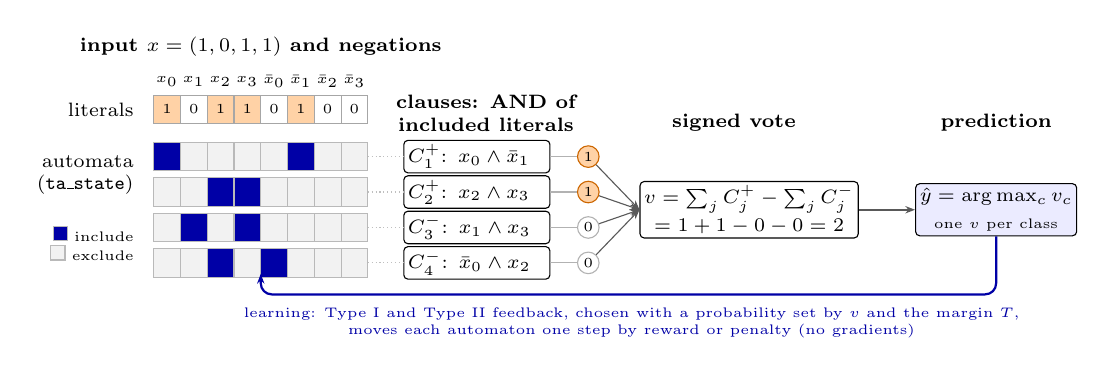
\begin{tikzpicture}[font=\scriptsize, x=1cm, y=1cm,
  cell/.style={draw=gray!55, minimum width=0.34cm, minimum height=0.36cm, inner sep=0pt, anchor=center},
  inc/.style={cell, fill=blue!65!black, text=white},
  exc/.style={cell, fill=gray!10},
  lit/.style={cell, draw=gray!70, fill=white, font=\tiny},
  lit1/.style={cell, draw=gray!70, fill=orange!35, font=\tiny},
  cbox/.style={draw, rounded corners=1.5pt, minimum height=0.32cm, inner sep=1.5pt, anchor=west, fill=white},
  arr/.style={-{Stealth[length=3.5pt]}, thick, gray!70!black},
  hdr/.style={font=\scriptsize\bfseries, anchor=south, align=center},
  side/.style={anchor=east, align=right, font=\scriptsize}]

  % ---- literals of the input --------------------------------------------------------
  \node[hdr] at (1.19,2.0) {input $x=(1,0,1,1)$ and negations};
  \foreach \k/\l in {0/x_0,1/x_1,2/x_2,3/x_3,4/\bar x_0,5/\bar x_1,6/\bar x_2,7/\bar x_3}{
    \node[font=\tiny] at (\k*0.34,1.8) {$\l$};
  }
  \foreach \v [count=\k from 0] in {1,0,1,1,0,1,0,0}{
    \ifnum\v=1 \node[lit1] at (\k*0.34,1.45) {1}; \else \node[lit] at (\k*0.34,1.45) {0}; \fi
  }
  \node[side] at (-0.3,1.45) {literals};

  % ---- one Tsetlin automaton per (clause, literal) ------------------------------------
  \foreach \row/\incl in {0/{0,5}, 1/{2,3}, 2/{1,3}, 3/{2,4}}{
    \pgfmathsetmacro{\yy}{0.85-\row*0.45}
    \foreach \k in {0,...,7}{
      \def\isin{0}
      \foreach \i in \incl {\ifnum\i=\k \xdef\isin{1}\fi}
      \ifnum\isin=1 \node[inc] at (\k*0.34,\yy) {}; \else \node[exc] at (\k*0.34,\yy) {}; \fi
    }
  }
  \node[side] at (-0.3,0.62) {automata\\(\code{ta\_state})};
  \node[side, font=\tiny] at (-0.3,-0.25)
    {\tikz\node[inc, minimum width=0.18cm, minimum height=0.18cm]{}; include\\[1pt]
     \tikz\node[exc, minimum width=0.18cm, minimum height=0.18cm]{}; exclude};

  % ---- clauses ------------------------------------------------------------------------
  \node[hdr] at (4.05,1.05) {clauses: AND of\\included literals};
  \foreach \row/\txt/\pol/\out in {0/{x_0 \wedge \bar x_1}/+/1, 1/{x_2 \wedge x_3}/+/1,
                                   2/{x_1 \wedge x_3}/-/0, 3/{\bar x_0 \wedge x_2}/-/0}{
    \pgfmathsetmacro{\yy}{0.85-\row*0.45}
    \node[cbox, text width=1.75cm] (c\row) at (3.0,\yy)
      {$C_{\the\numexpr\row+1\relax}^{\pol}$: $\txt$};
    \draw[gray!50, densely dotted] (2.55,\yy) -- (c\row.west);
    \ifnum\out=1
      \node[circle, draw=orange!80!black, fill=orange!35, inner sep=1.1pt, font=\tiny] (o\row) at (5.35,\yy) {1};
    \else
      \node[circle, draw=gray!60, fill=white, inner sep=1.1pt, font=\tiny] (o\row) at (5.35,\yy) {0};
    \fi
    \draw[gray!60] (c\row.east) -- (o\row);
  }

  % ---- signed vote and prediction ------------------------------------------------------
  \node[hdr] at (7.2,1.05) {signed vote};
  \node[cbox, align=center] (v) at (6.0,0.175)
    {\mbox{$v = \sum_j C^{+}_j - \sum_j C^{-}_j$}\\[2pt] $= 1 + 1 - 0 - 0 = 2$};
  \foreach \row in {0,...,3}{ \draw[arr, thin] (o\row) -- (v.west); }
  \node[cbox, align=center, fill=blue!8] (p) at (9.5,0.175)
    {$\hat y = \arg\max_c v_c$\\[2pt] \tiny one $v$ per class};
  \node[hdr] at (p.north |- 0,1.05) {prediction};
  \draw[arr] (v.east) -- (p.west);

  % ---- learning: feedback to the automata ----------------------------------------------
  \draw[arr, blue!65!black, rounded corners=4pt] (p.south) |- (1.19,-0.9) -- (1.19,-0.64);
  \node[font=\tiny, text=blue!65!black, anchor=north, align=center] at (5.9,-0.95)
    {learning: Type~I and Type~II feedback, chosen with a probability set by $v$ and the margin $T$,\\
     moves each automaton one step by reward or penalty (no gradients)};
\end{tikzpicture}

\caption{A Tsetlin machine at a glance: each row of automata defines a clause, matching
  clauses vote with their polarity, and feedback moves the automata.}
\label{fig:tm}
\end{figure}

The reference software implements each variant as a C or CUDA kernel behind a
\code{fit}/\code{predict} interface~\citep{software_pytsetlinmachine,
software_pytsetlinmachinecuda,software_tmu}. For PyTorch~\citep{paszke2019pytorch} users this
leaves four gaps:
\emph{(i)}~the learned state sits in a private buffer that tensor tools cannot inspect, mask or
save; \emph{(ii)}~the device is fixed by the imported package, so CPU and GPU runs follow
different code paths; \emph{(iii)}~Booleanised data must leave the framework as NumPy arrays;
and \emph{(iv)}~a new feedback rule or output layer means a new kernel. \lib\ closes these gaps
with tensor-state \code{nn.Module}s, batched GPU feedback, one learning loop for flat,
convolutional and dense inputs, and an end-to-end workflow from Booleanisation to rules.

% ===========================================================================
\section{Design}
\label{sec:design}

\paragraph{State as tensors.}
A machine with $C$ clauses over $F$ features holds the automata of Figure~\ref{fig:tm} as an
integer buffer \code{ta\_state} of shape $(C, 2F)$, with memory depth $N$.
The counters are buffers, not parameters, so \code{to()}, \code{state\_dict()} and lazy shape
inference (as in \code{LazyLinear}) work unchanged. Learning is \code{update(x, y)}, the analogue
of \code{loss.backward(); optimizer.step()}, which returns the pre-update vote sums for logging;
the empty-clause convention (output~1 while learning, 0 while predicting) follows
\code{train()}/\code{eval()}.

\paragraph{One learning loop, many input structures.}
The package has four layers. \code{functional} holds all learning
maths as stateless tensor operations, and \code{TsetlinMachineBase} runs the generic loop. A concrete
model supplies only an output layer and a feedback policy through three hooks. A new input
structure overrides encoding, clause evaluation and feedback counting: one mixin turns every
flat model into a convolutional one, in which a clause fires if it matches any patch and
positions are thermometer-encoded~\citep{granmo2019convolutional}; a 3-D subclass changes only
the patch geometry; and dense segmentation folds pixels into the batch axis so that each is a
flat example. No variant re-implements learning.


\paragraph{Batched feedback.}
Classically, every training example triggers a stochastic pass over all $C\times 2F$ automata.
For a mini-batch of $B$ examples, \lib\ evaluates all clauses at once and draws the per-example
clause selections for feedback with the usual probability $(T \mp \mathrm{clip}(v,-T,T))/2T$
for vote sum $v$ and margin $T$. With $S_{\mathrm{I}}, S_{\mathrm{II}} \in \{0,1\}^{B\times C}$
the Type~I and Type~II selections of firing clauses, $\bar S_{\mathrm{I}}$ the Type~I selections
of non-firing clauses and $L \in \{0,1\}^{B\times 2F}$ the literals, the feedback events are
counted with matrix products,
\begin{equation*}
  n^{\mathrm{true}} = S_{\mathrm{I}}^{\top} L,\quad
  n^{\mathrm{false}} = S_{\mathrm{I}}^{\top} (1-L),\quad
  n^{\mathrm{II}} = S_{\mathrm{II}}^{\top} (1-L),\quad
  n^{\mathrm{Ib}} = \bar S_{\mathrm{I}}^{\top}\mathbf{1}.
\end{equation*}
Each event is an independent Bernoulli trial, so the aggregate transition is drawn in closed
form and committed once per batch:
\begin{equation*}
  \Delta = \mathrm{Bin}\bigl(n^{\mathrm{true}}, p_{\mathrm{mem}}\bigr)
  - \mathrm{Bin}\bigl(n^{\mathrm{false}} + n^{\mathrm{Ib}}\mathbf{1}^{\top}, 1/s\bigr)
  + \min\bigl(n^{\mathrm{II}}, \max(N - \mathrm{state}, 0)\bigr),
\end{equation*}
with specificity $s$ and $p_{\mathrm{mem}} = (s-1)/s$, or $1$ with boosted true-positive
feedback. At $B=1$ this is the classical update term by term; for $B>1$ it approximates it as
mini-batch SGD approximates SGD~\citep{bottou2018optimization}, and
\code{feedback\_mode="sequential"} keeps the exact path. Because one commit can include many
literals, the clause-size budget~\citep{abeyrathna2023clausesize} is a hard cap enforced at
commit.

% ===========================================================================
\section{Functionality and Usage}
\label{sec:usage}

Listing~\ref{lst:xor} shows the complete workflow on Noisy XOR~\citep{granmo2018tsetlin}: with
40\% label noise the machine recovers and prints the generating rule. Version \ph{0.3.x} ships
\code{TsetlinMachine} (optional clause weights~\citep{phoulady2019weighted}),
\code{CoalescedTsetlinMachine} (multi-class or multi-label) and \code{RegressionTsetlinMachine},
convolutional 1-D, 2-D and 3-D variants of each, and dense segmentation machines. Booleanisation
encoders (thermometer, hypervector~\citep{halenka2024hypervectors} and others) are \code{nn.Module}s that run on the model's device and carry feature names
into the rules (\code{worst\_perimeter>=105.9} rather than \code{x37}). A \code{Trainer} with
callbacks accepts tensors and \code{DataLoader}s, and the interpretation tools extract rules
and global, local and per-pixel importance~\citep{blakely2020closedform}. The package is pure Python (PyTorch $\ge 2.0$, NumPy).

\begin{lstlisting}[style=py, float=t, caption={Training, evaluating and reading a Tsetlin machine on Noisy XOR.}, label={lst:xor}]
import torchtsetlin as tt
x_train, y_train = tt.data.make_noisy_xor(5000, noise=0.4)   # Boolean features, int labels
x_test,  y_test  = tt.data.make_noisy_xor(2000, noise=0.0, seed=1)
model = tt.TsetlinMachine(n_features=12, n_classes=2, n_clauses=20, T=15, s=3.9).to("cuda")
trainer = tt.Trainer(model, batch_size=10, callbacks=[tt.EarlyStopping(patience=20)])
trainer.fit((x_train, y_train), epochs=100, val_data=(x_test, y_test))
print(trainer.evaluate((x_test, y_test)))   # {'accuracy': ...}
print(model.rules()[:2])  # ['IF x0 AND NOT x1 THEN 1', 'IF x1 AND NOT x0 THEN 1']
\end{lstlisting}

% ===========================================================================
\section{Comparison with Existing Software}
\label{sec:comparison}

Table~\ref{tab:compare} compares \lib\ with the maintained TM packages.
\code{pyTsetlinMachine}~\citep{software_pytsetlinmachine} and
\code{PyTsetlinMachineCUDA}~\citep{software_pytsetlinmachinecuda} implement one class per
variant in C and CUDA; \code{tmu}~\citep{software_tmu} unifies them over reusable clause and
weight banks with CPU and CUDA backends; \code{green-tsetlin}~\citep{software_greentsetlin,greentsetlin2024}
targets efficient CPU training and deployment. Every GPU path among them is a hand-written
PyCUDA kernel. All keep the automata in a native buffer; \lib\
alone builds on a general-purpose tensor library, trading some kernel-level speed on small CPU
workloads for device portability, interoperability and extensibility in Python.

\begin{table}[t]
\centering\footnotesize
\setlength{\tabcolsep}{3.5pt}
\caption{Comparison with TM software, latest PyPI releases \ph{as of submission} (\cmark\ yes,
  \pmark\ partial, \xmark\ no; red: not yet verified or measured). Bottom: MNIST~\citep{lecun1998mnist},
  \res{2000 clauses, batch 256; hardware}.}
\label{tab:compare}
\begin{tabular}{@{}lccccc@{}}
\toprule
 & \code{pyTsetlinMachine} & \code{PyTMCUDA} & \code{tmu} & \code{green-tsetlin} & \lib \\
\midrule
Backend                           & C        & PyCUDA     & C\,/\,PyCUDA & C++    & PyTorch \\
CPU and GPU from one class        & \xmark   & \xmark     & \cmark     & \xmark   & \cmark \\
Conv.\ 1-D\,/\,2-D\,/\,3-D        & \xmark\,\cmark\,\xmark & \xmark\,\cmark\,\xmark & \xmark\,\cmark\,\xmark & \ph{?} & \cmark\,\cmark\,\cmark \\
Regression\,/\,coalesced          & \cmark\,\xmark & \cmark\,\xmark & \cmark\,\cmark & \xmark\,\xmark & \cmark\,\cmark \\
Dense segmentation                & \xmark   & \xmark     & \xmark     & \xmark   & \cmark \\
Tensor state, \code{state\_dict}  & \xmark   & \xmark     & \xmark     & \xmark   & \cmark \\
New variant without C/CUDA        & \xmark   & \xmark     & \pmark     & \xmark   & \cmark \\
Unit tests and CI                 & \xmark   & \xmark     & \cmark     & \cmark   & \cmark \\
\midrule
MNIST epoch, CPU / GPU (s)        & \res{0.0} / --  & -- / \res{0.0} & \res{0.0} / \res{0.0} & \res{0.0} / -- & \res{0.0} / \res{0.0} \\
Peak GPU memory (MiB)             & --        & \res{0}   & \res{0}    & --        & \res{0} \\
MNIST test accuracy (\%)          & \res{0.0} & \res{0.0} & \res{0.0}  & \res{0.0} & \res{0.0} \\
\bottomrule
\end{tabular}
\end{table}

% ===========================================================================
\section{Performance and Fidelity}
\label{sec:performance}

For a 784-feature machine with \res{500} clauses per class (Figure~\ref{fig:bench}a), GPU
throughput grows from \res{$a$} examples/s at $B=1$ to
\res{$b$} at $B=4096$; at $B=256$ the same code runs \res{$c\times$} faster on an \ph{RTX~3090}
than on a \ph{16-core CPU}, up to \res{$e\times$} for the clause counts of the image literature.
Batching is an approximation, so Figure~\ref{fig:bench}b measures its cost: on Noisy XOR,
batches up to about \res{50} stay in the accuracy band of the exact sequential algorithm and
batch \res{200} degrades, which motivates the recommended \res{16--64} (flat) and \res{8--32}
(convolutional). One command, \code{benchmarks/run\_benchmarks.sh},
reproduces every number and figure on other hardware.

\begin{figure}[t]
\centering
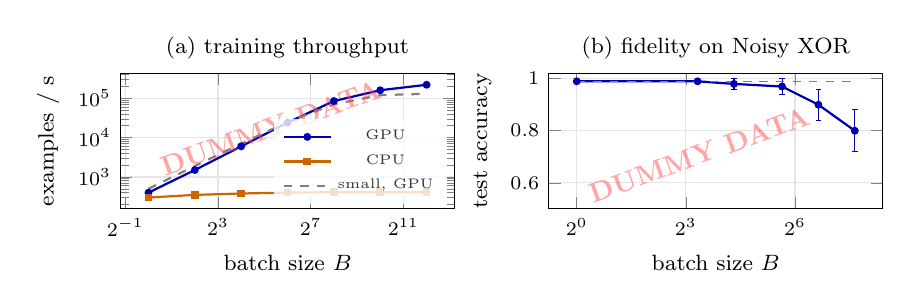
\begin{tikzpicture}
\begin{axis}[name=thr, width=0.48\linewidth, height=3.3cm, xmode=log, ymode=log, log basis x=2,
  xlabel={batch size $B$}, ylabel={examples / s}, title={\footnotesize (a) training throughput},
  tick label style={font=\scriptsize}, label style={font=\footnotesize},
  legend style={font=\tiny, at={(0.98,0.03)}, anchor=south east, draw=none, fill=white, fill opacity=0.8},
  grid=major, grid style={gray!20}, title style={yshift=-1ex}]
  % DUMMY DATA - shape only
  \addplot[thick, blue!70!black, mark=*, mark size=1pt] coordinates
    {(1,400) (4,1500) (16,6000) (64,24000) (256,85000) (1024,160000) (4096,220000)};
  \addlegendentry{GPU}
  \addplot[thick, orange!80!black, mark=square*, mark size=1pt] coordinates
    {(1,300) (4,350) (16,380) (64,400) (256,410) (1024,410) (4096,410)};
  \addlegendentry{CPU}
  \addplot[thick, dashed, gray] coordinates
    {(1,500) (4,1900) (16,7000) (64,25000) (256,70000) (1024,120000) (4096,130000)};
  \addlegendentry{small, GPU}
  \node[red!70, rotate=20, font=\bfseries, opacity=0.5] at (rel axis cs:0.45,0.6) {DUMMY DATA};
\end{axis}
\begin{axis}[at={(thr.east)}, anchor=west, xshift=1.2cm, width=0.48\linewidth, height=3.3cm,
  xmode=log, log basis x=2, xlabel={batch size $B$}, ylabel={test accuracy},
  title={\footnotesize (b) fidelity on Noisy XOR}, ymin=0.5, ymax=1.02,
  tick label style={font=\scriptsize}, label style={font=\footnotesize}, grid=major,
  grid style={gray!20}, title style={yshift=-1ex}]
  % DUMMY DATA - shape only: mean +- sd over 3 seeds; B=1 is the exact sequential algorithm
  \addplot[thick, blue!70!black, mark=*, mark size=1pt,
    error bars/.cd, y dir=both, y explicit] coordinates
    {(1,0.99) +- (0,0.01) (10,0.99) +- (0,0.01) (20,0.98) +- (0,0.02) (50,0.97) +- (0,0.03)
     (100,0.90) +- (0,0.06) (200,0.80) +- (0,0.08)};
  \addplot[dashed, gray, domain=1:200] {0.99};
  \node[red!70, rotate=20, font=\bfseries, opacity=0.5] at (rel axis cs:0.45,0.4) {DUMMY DATA};
\end{axis}
\end{tikzpicture}
\caption{(a) Throughput, same code on GPU and CPU. (b) Noisy XOR accuracy over \res{3} seeds;
  $B=1$ is the exact sequential algorithm.}
\label{fig:bench}
\end{figure}

% ===========================================================================
\section{Software Quality and Community}
\label{sec:quality}

The suite has \res{$n$} tests with \res{$p$\%} line coverage; device-dependent tests run on the
CPU and on CUDA when present. It also pins behaviour that breaks silently, such as
empty-clause semantics and the hard clause budget under batched commits. Continuous
integration lints and tests on Python 3.9, 3.11 and 3.12 \ph{on Linux, macOS and Windows};
releases go to PyPI by Trusted Publishing. The
documentation\footnote{\url{https://vajira.info/torchtsetlin/}} offers guides, examples, an API
reference, and an SQL-queryable catalogue of \res{$r$} results on
\res{$d$} datasets from \res{$m$} TM papers. Development is open on GitHub
(\url{https://github.com/vlbthambawita/torchtsetlin}, MIT licence).

\acks{\ph{Funding sources and grant numbers.} The author declares no competing interests.}

\bibliography{references}

\end{document}
